% ################################
\section{Úvod}

Zde vysvětlit problémovou situaci a otázky, které se budou v bakalářské/diplomové práci řešit.


% ################################
\section{Cíl a metodika práce}

Smysl a účel, výzkumné otázky.  

Cíle, hypotézy/výzkumné otázky, způsob hledání odpovědí na výzkumné otázky včetně metodiky vlastního výzkumu/šetření, literární rešerše.


% ################################
\section{Kapitola -- Vlastní text práce}

Vlastní řešení dokládá student zpravidla v několika kapitolách. Podle charakteru práce musí student uvážit, zda informace netextové povahy (data, tabulky, obrázky atd.) bude uvádět přímo v textu, nebo je zařadí až za celou práci ve formě příloh, či bude kombinovat oba způsoby. 

Více podrobností viz Metodické pokyny pro vypracování bakalářských a diplomových prací (zveřejňované formou výnosů děkana) a v kurzu MES -- Metodologický seminář. \cite{autor00}

\subsection{Podkapitola}

Vlastní text práce.

\begin{table}[htb!]  
\caption{Název tabulky.}

\begin{tabular}{| l | l | l | l |}
\hline
 \hspace{0.22\textwidth} & \hspace{0.22\textwidth} & \hspace{0.22\textwidth} & \hspace{0.22\textwidth} \\
\hline
 & & & \\
\hline
 & & & \\
\hline
 & & & \\
\hline
\end{tabular} \\

Zdroj: citace zdroje, nebo autor, vlastní zpracování
%\label{tab:empty}
\end{table}

\subsubsection{Podřazená podkapitola}

Vlastní text práce.

\begin{figure}[htb!]
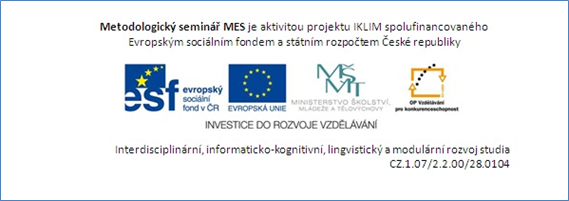
\includegraphics{img/MES.png}
\caption{Název obrázku/grafu/fotografie.}
Zdroj: citace zdroje, nebo autor, vlastní zpracování
%\label{fig:MES}
\end{figure} 


% ################################
\section{Shrnutí a diskuse výsledků}

Souhrn a diskuse vlastních výsledků získaných v průběhu řešení problému. 


% ################################
\section{Závěry a doporučení}

Kritická diskuse nad výsledky, ke kterým autor dospěl (soulad výsledků s literaturou či předpoklady; výsledky a okolnosti, které zvláště ovlivnily předkládanou práci atd.). Je vhodné naznačit i případné další (popř. alternativní) možnosti zkoumání dané problematiky a otevřené problémy pro další studium.
